 \begin{frame} \frametitle{Wavelet transforms for EXAFS analysis}

  \begin{itemize}
  \item  Can we fit EXAFS data in wavelet space?   {\RedEmph{Yes, we can}}.
  \item  Can we learn anything from wavelet  transforms?  {\RedEmph{Maybe\ldots}}
  \end{itemize}

  \vmm
  \hrule
  \vmm

{\only<1,2,3>{ Fits to FeO first 2 shells fitting in ``wavelet space'':}}

% {\only<4,5>{ The uncertainty in FeO data in ``wavelet space'':}}


{\only<1>{
\begin{columns}
  \begin{column}[T]{60mm}
    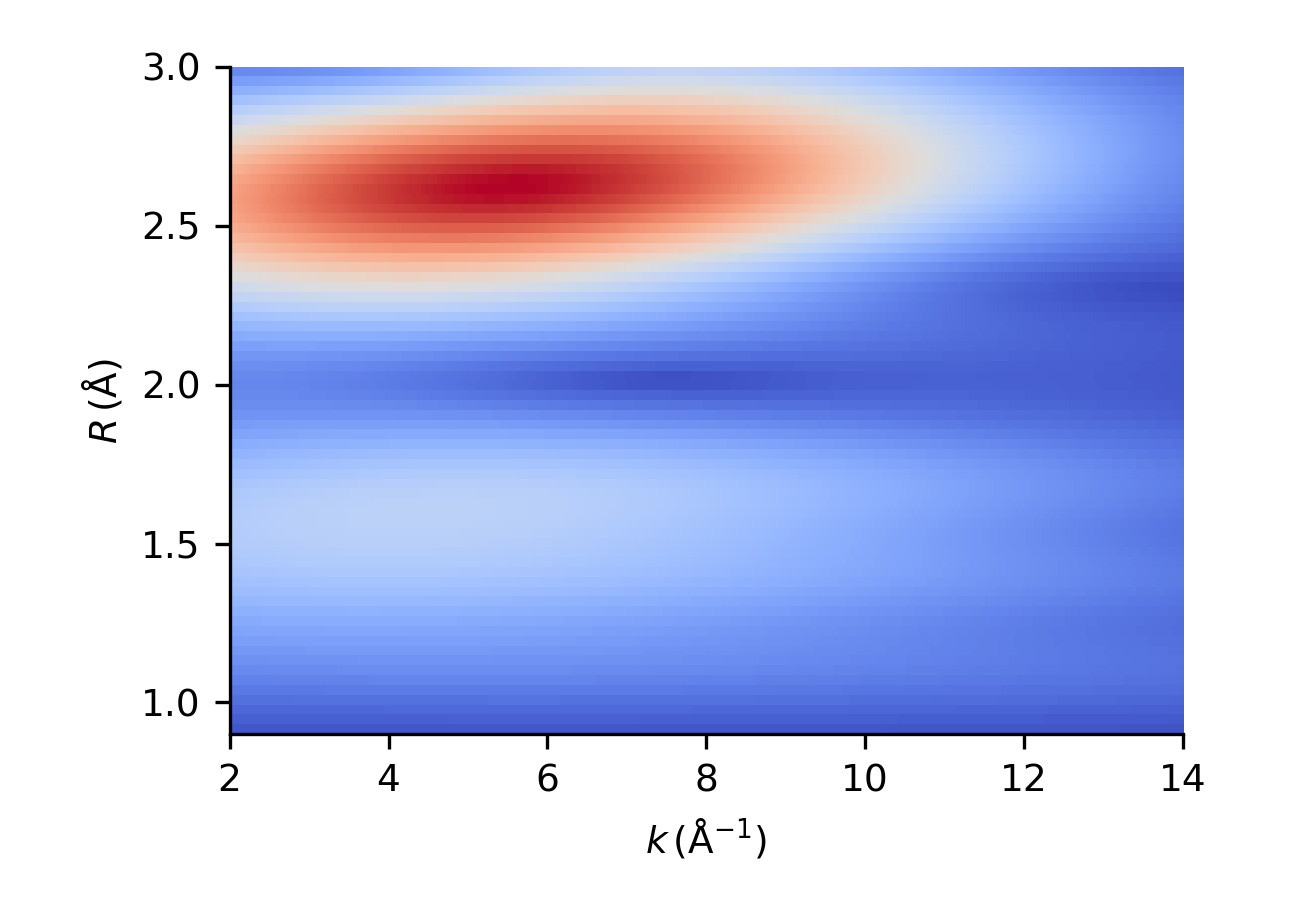
\includegraphics[width=57mm]{figs/wavelets/feo_cwt_data_mag}

    \hspace{5mm} FeO data, magnitude of wavelet
  \end{column}
  \begin{column}[T]{60mm}
    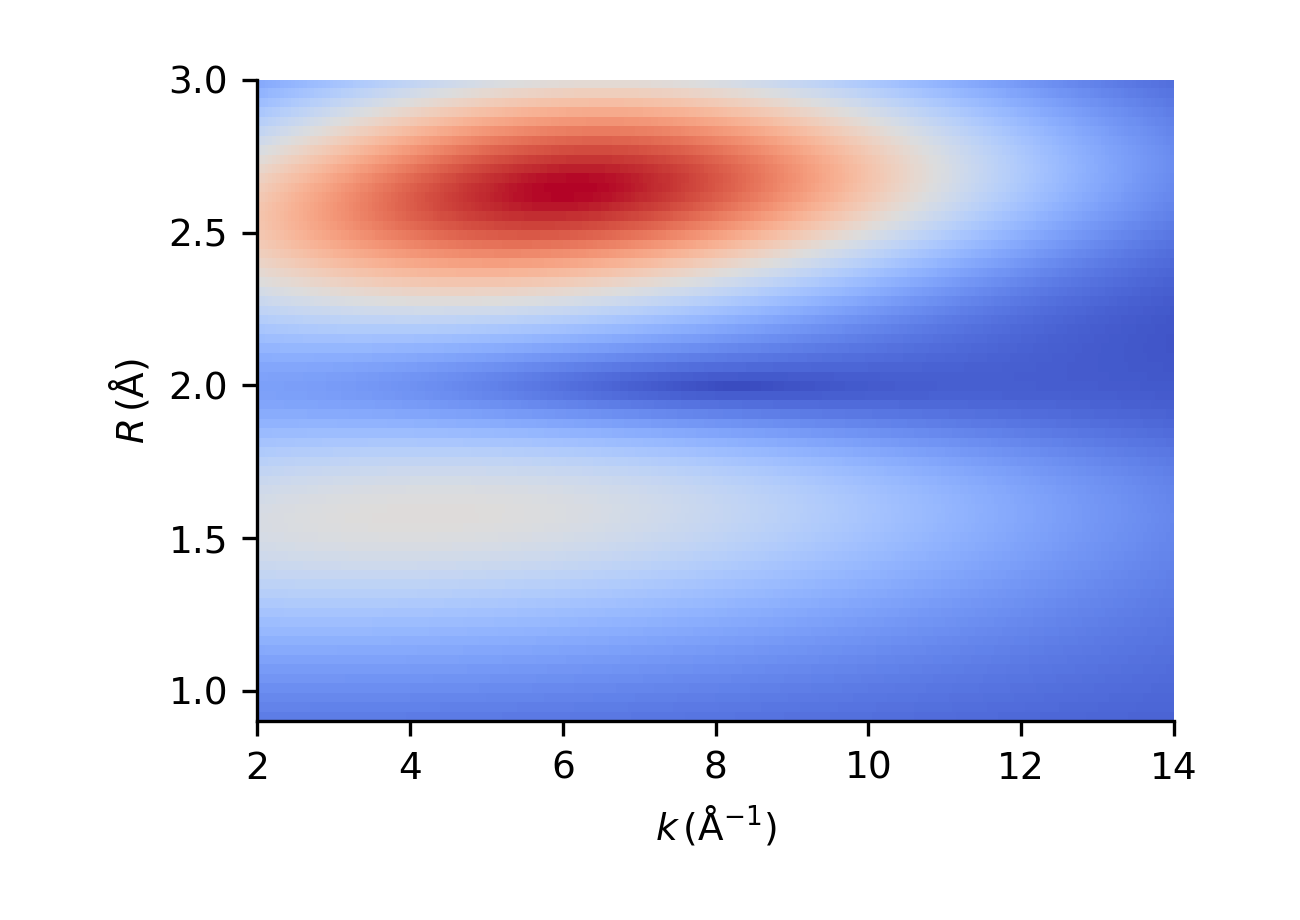
\includegraphics[width=57mm]{figs/wavelets/feo_cwt_model_mag}

    \hspace{5mm} FeO model, magnitude of wavelet

  \end{column}
\end{columns}

}}

{\only<2>{
\begin{columns}
  \begin{column}[T]{60mm}
    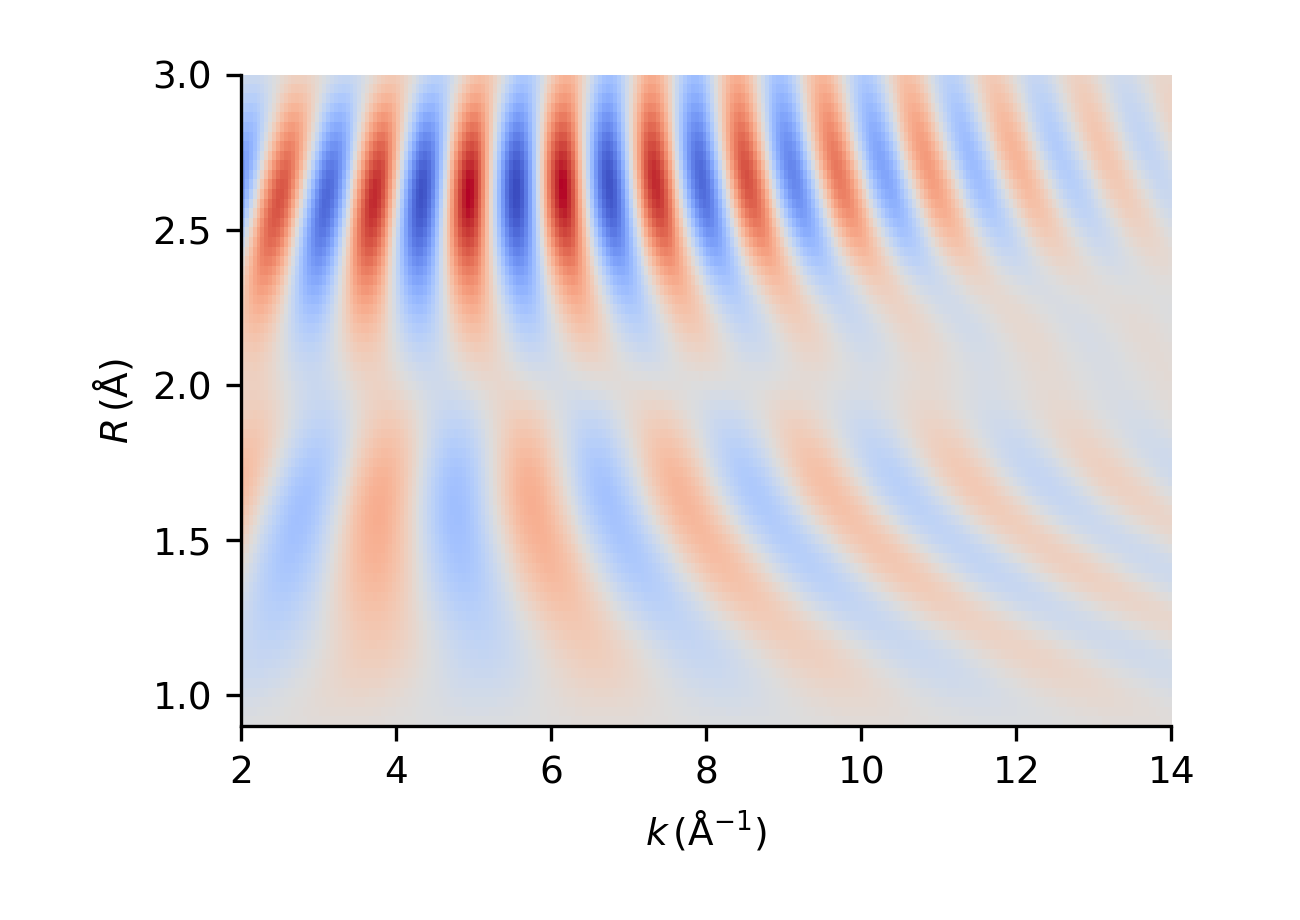
\includegraphics[width=57mm]{figs/wavelets/feo_cwt_data_re}

    \hspace{5mm} FeO data, real part of wavelet
  \end{column}
  \begin{column}[T]{60mm}
    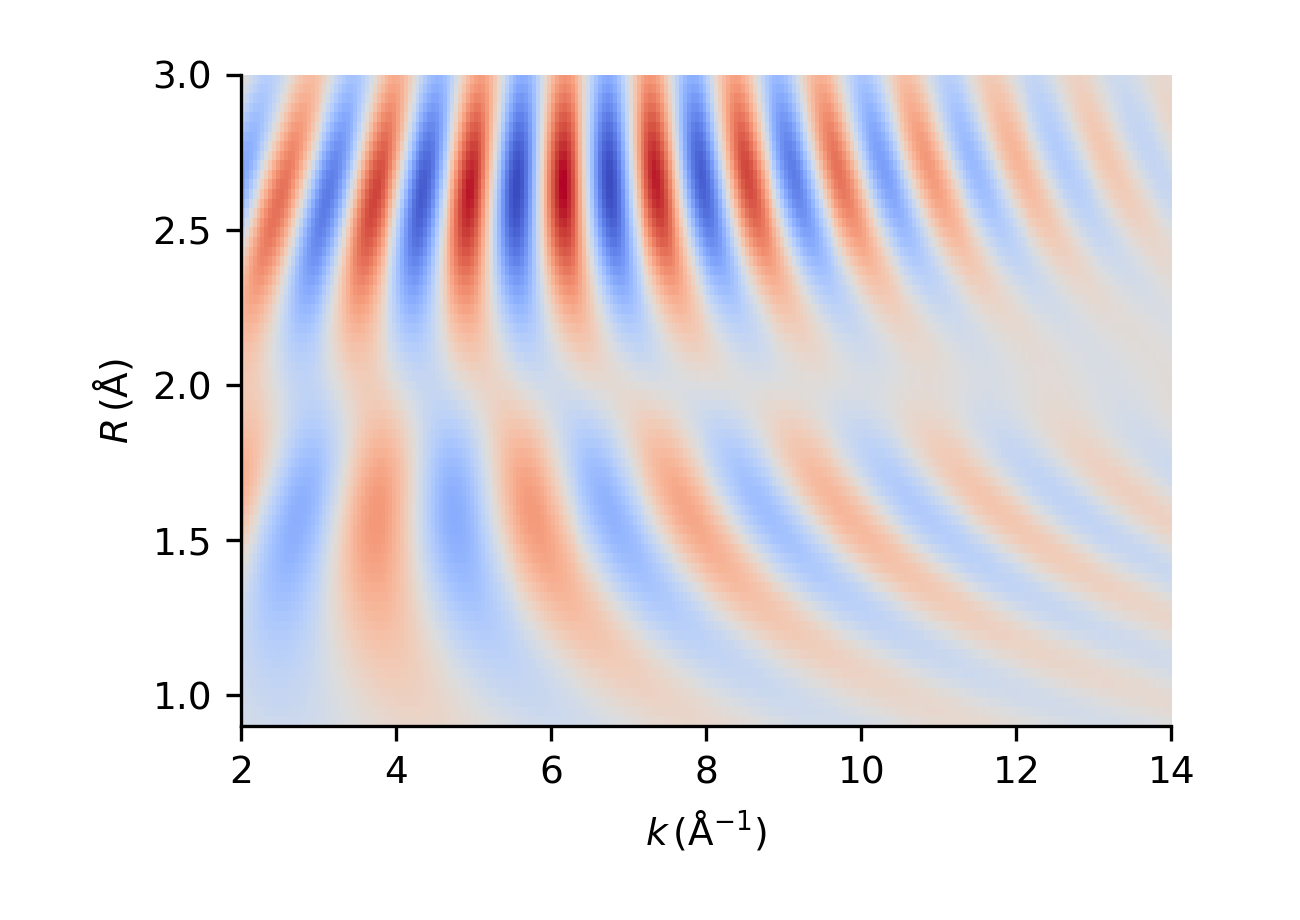
\includegraphics[width=57mm]{figs/wavelets/feo_cwt_model_re}

    \hspace{5mm} FeO model, real part of wavelet

  \end{column}
\end{columns}

}}


{\only<3>{
\begin{columns}
  \begin{column}[T]{60mm}
    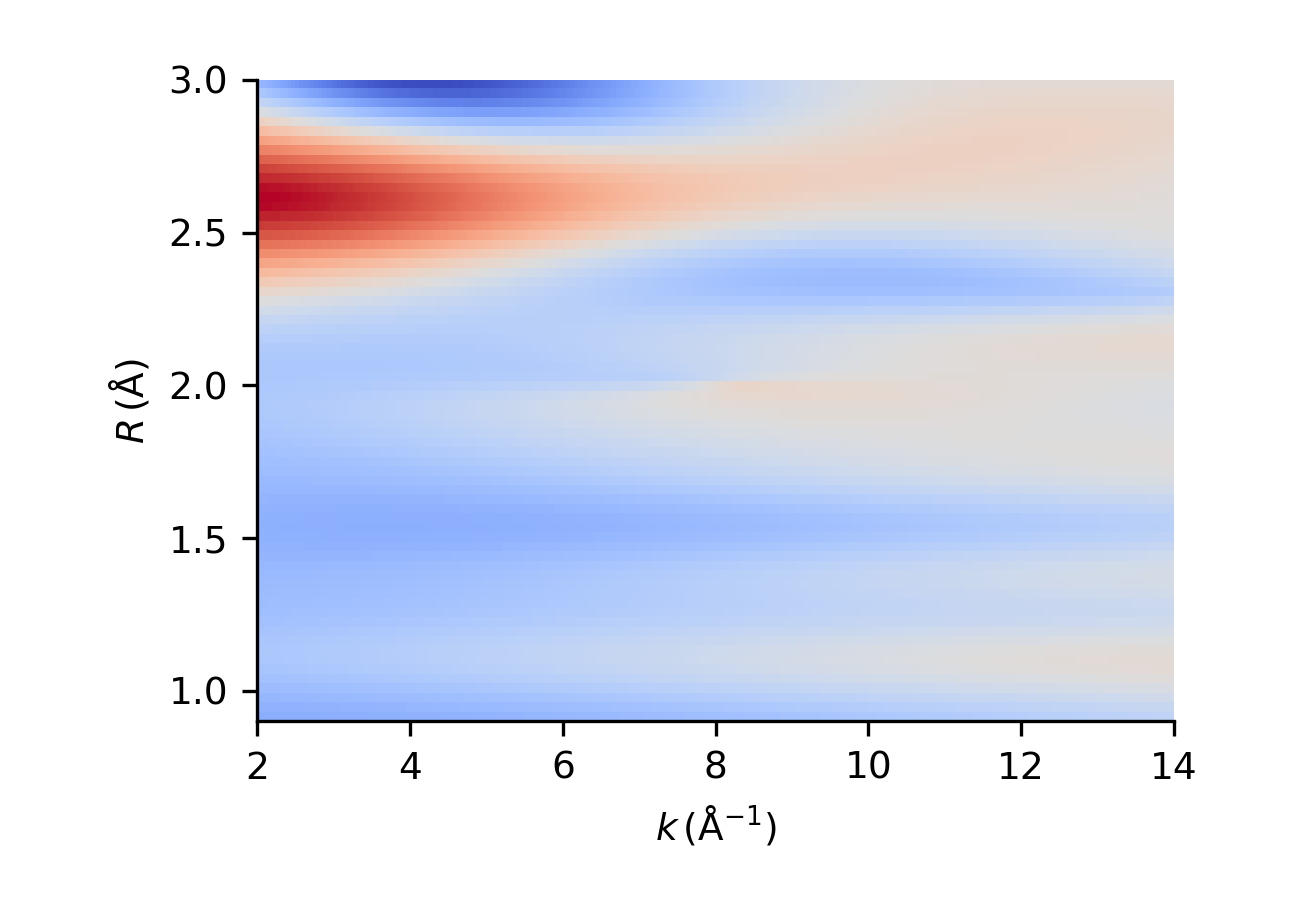
\includegraphics[width=57mm]{figs/wavelets/feo_cwt_misfit_mag}

    \hspace{5mm} FeO (data-model), magnitude
  \end{column}
  \begin{column}[T]{60mm}
    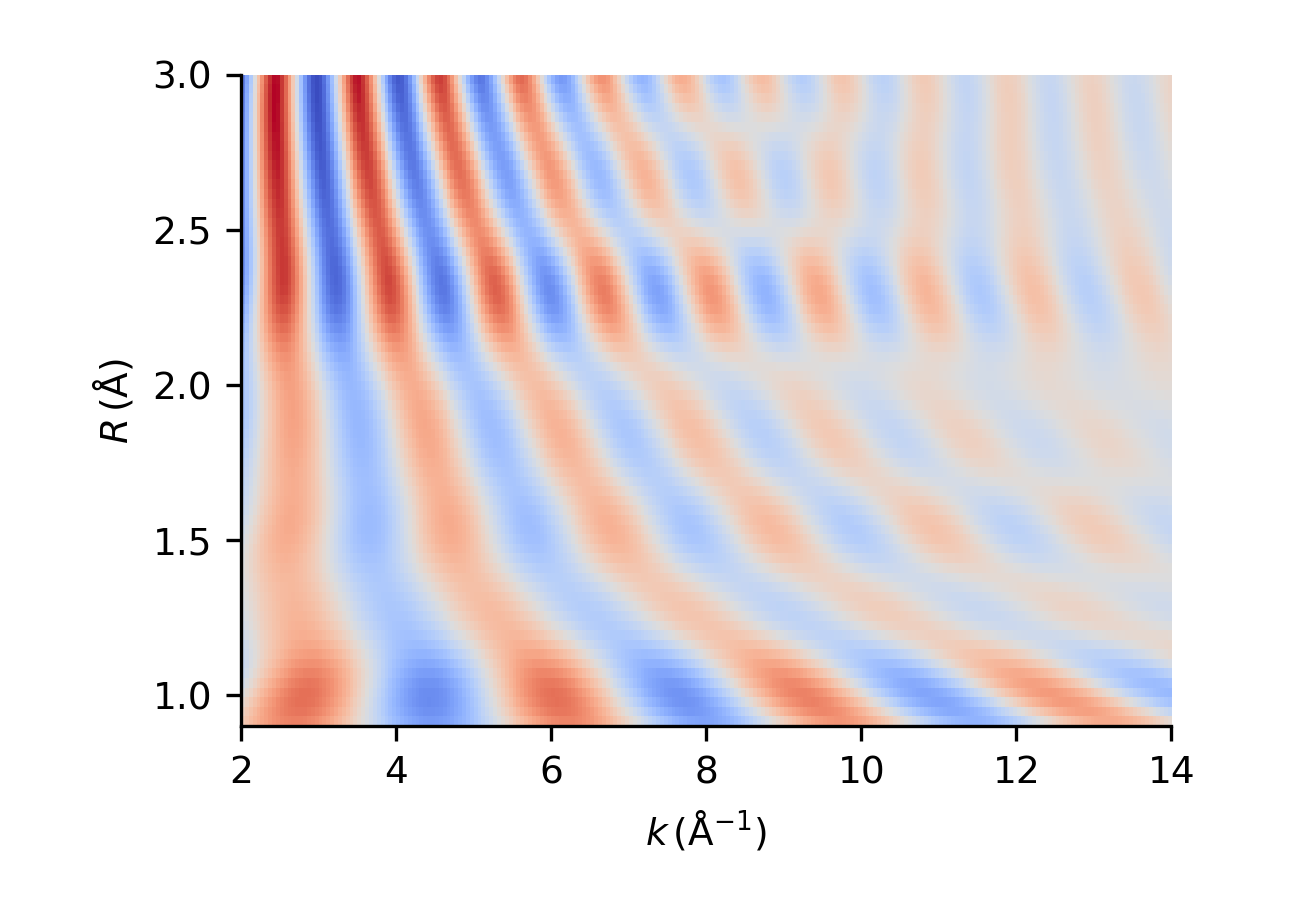
\includegraphics[width=57mm]{figs/wavelets/feo_cwt_misfit_re}

    \hspace{5mm} FeO (data-model), real part

  \end{column}
\end{columns}

}}



% {\only<4>{
% \begin{columns}
%   \begin{column}[T]{60mm}
%     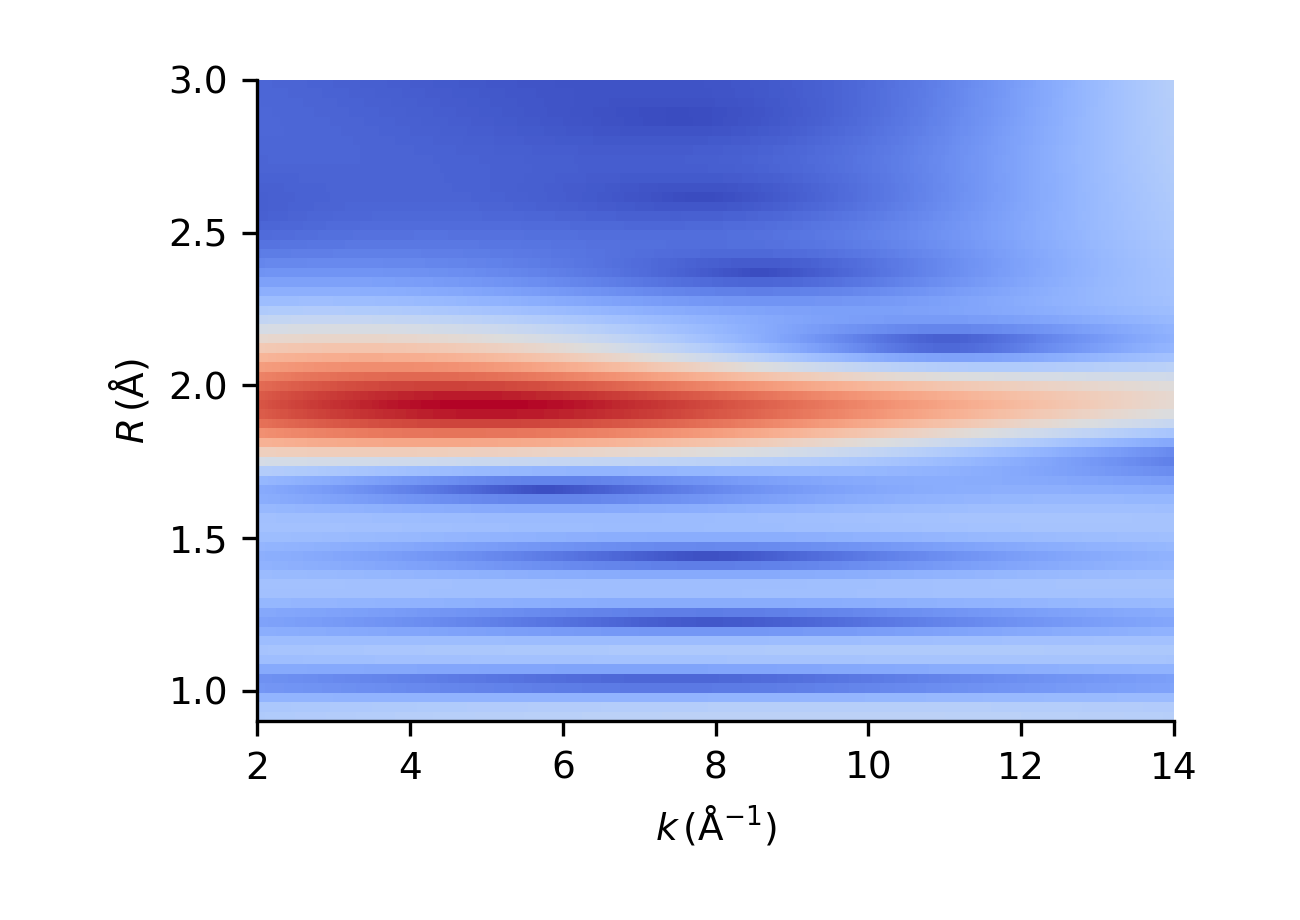
\includegraphics[width=57mm]{figs/wavelets/feo_cwt_delchi_mag}

%     \hspace{5mm} FeO uncertainty:  magnitude  of wavelet
%   \end{column}
%   \begin{column}[T]{60mm}
%     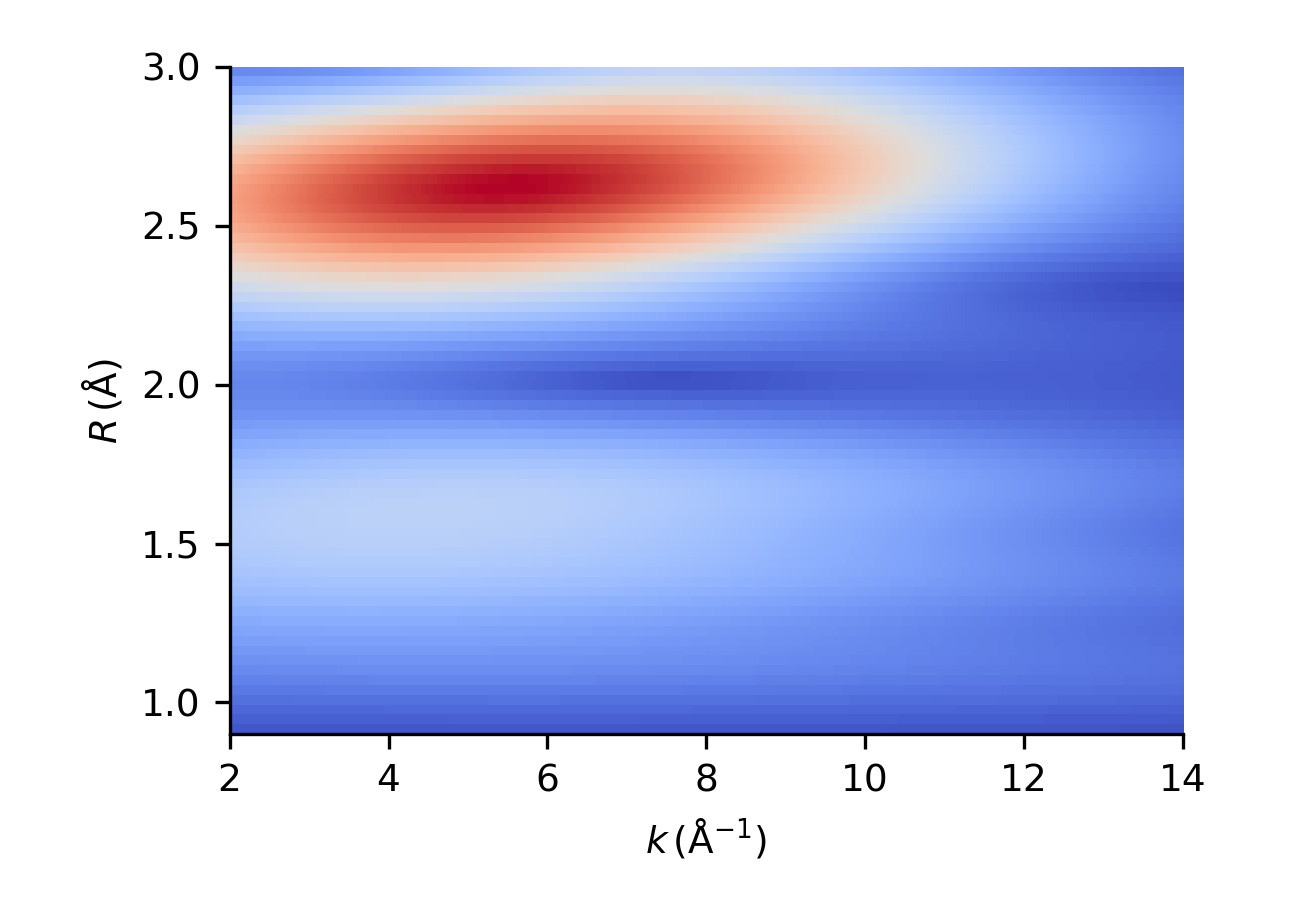
\includegraphics[width=57mm]{figs/wavelets/feo_cwt_data_mag}

%     \hspace{5mm} FeO data: magnitude  of wavelet

%   \end{column}
% \end{columns}

% }}

% {\only<5>{
% \begin{columns}
%   \begin{column}[T]{60mm}
%     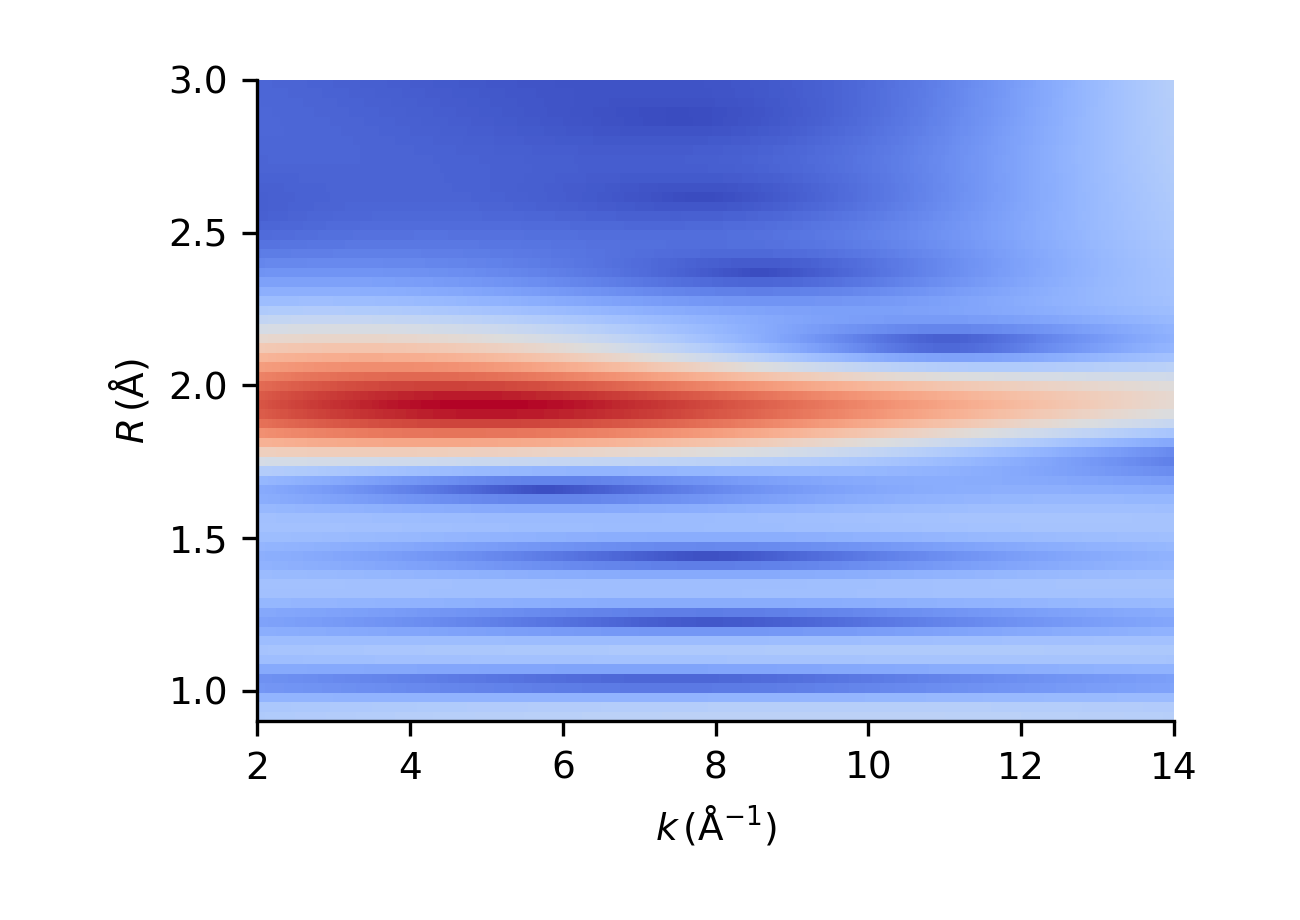
\includegraphics[width=57mm]{figs/wavelets/feo_cwt_delchi_mag}

%     \hspace{5mm} FeO uncertainty:  magnitude  of wavelet
%   \end{column}
%   \begin{column}[T]{60mm}
%     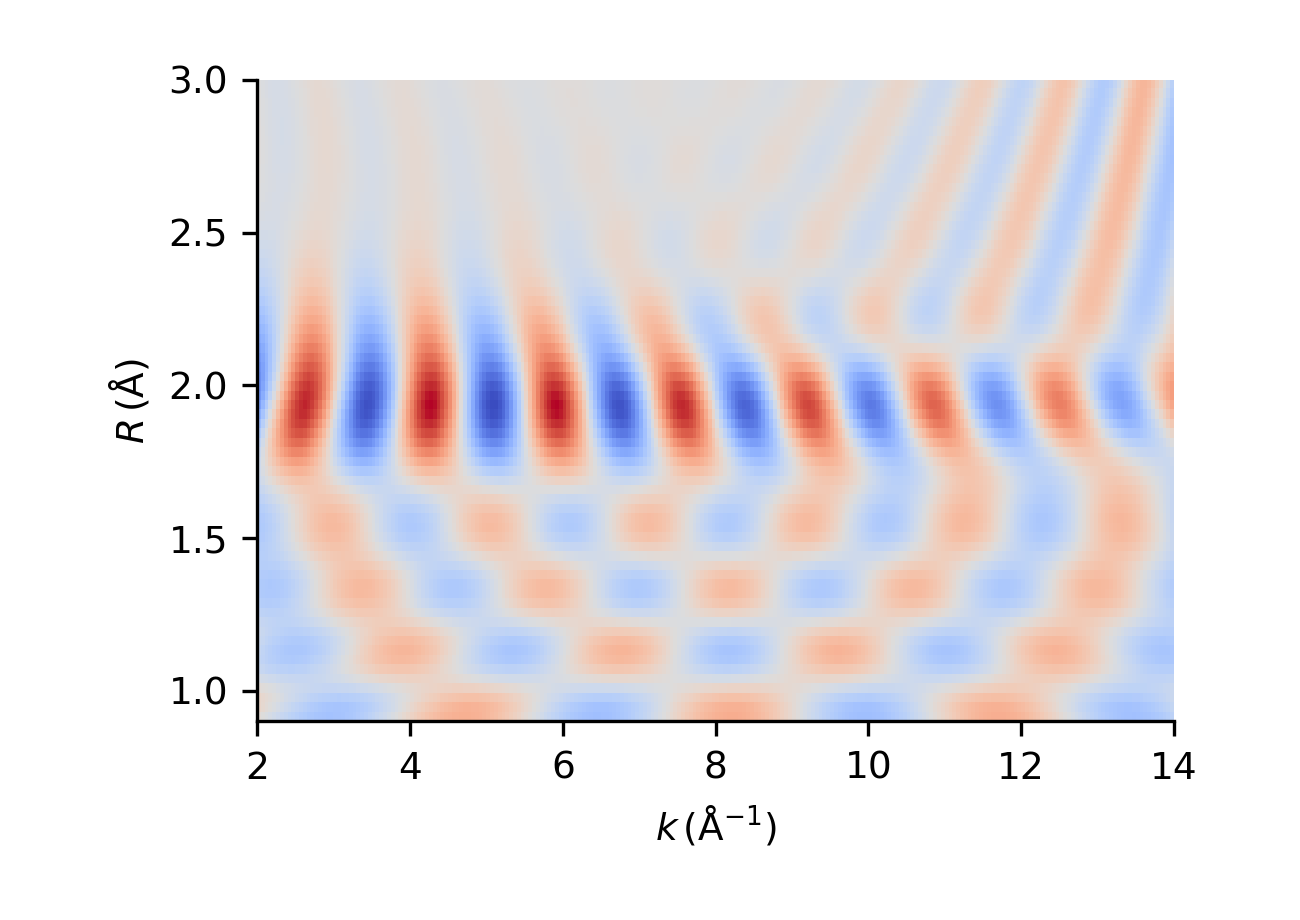
\includegraphics[width=57mm]{figs/wavelets/feo_cwt_delchi_re}

%     \hspace{5mm} FeO uncertainty: real part of wavelet

%   \end{column}
% \end{columns}

% }}


% % {\only<6>{
% \begin{columns}
%   \begin{column}[T]{60mm}
%     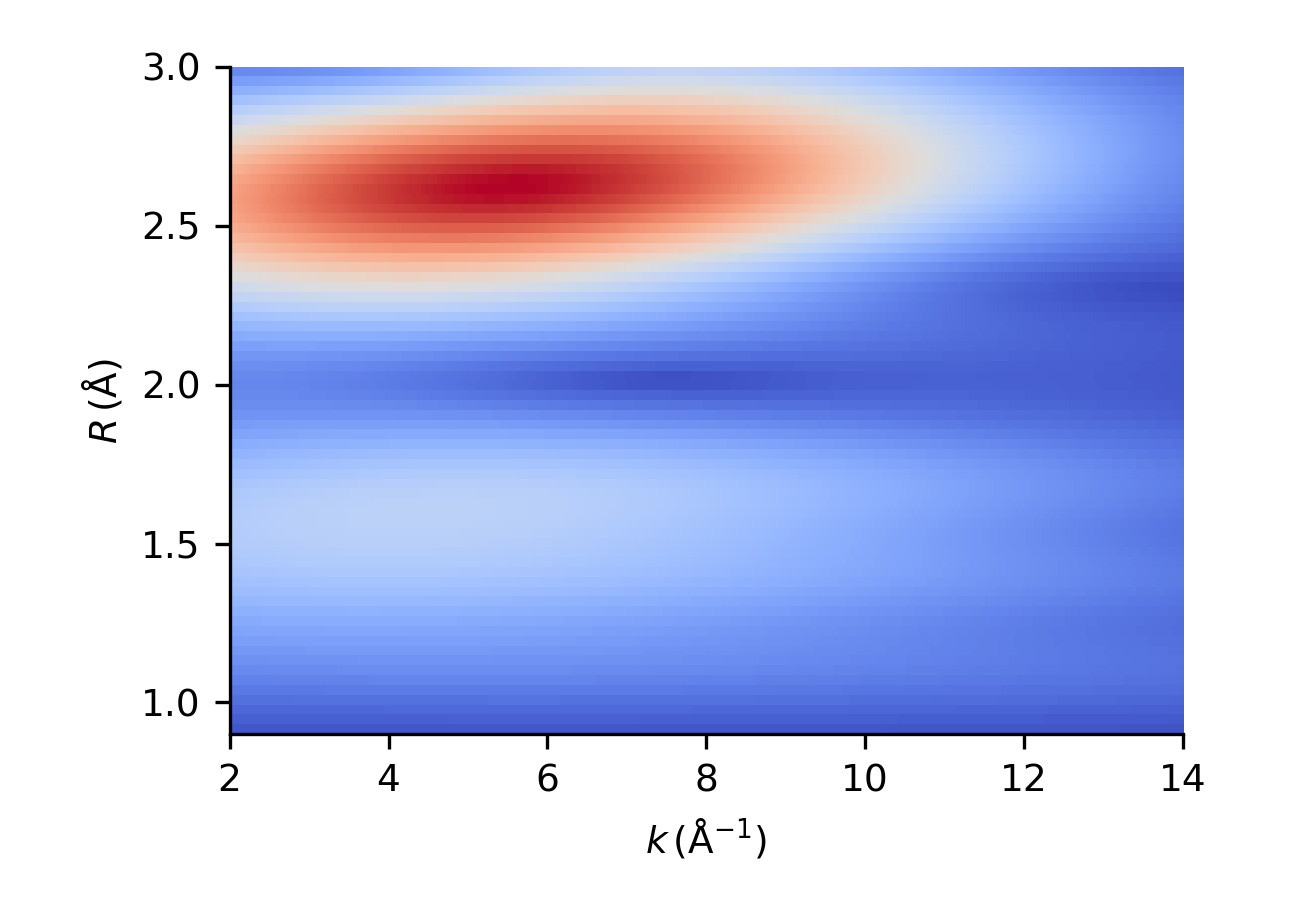
\includegraphics[width=57mm]{figs/wavelets/feo_cwt_data_mag}

%     \hspace{5mm} FeO data, magnitude of wavelet
%   \end{column}
%   \begin{column}[T]{60mm}

%     \vmm\vmm\vmm

%     These ``wavelet fits'' use a rectangular window in $k$ and $R$, similar
%     to that used when fitting $R$-space: $k=[2, 14]\rm\AA^{-1}$,
%     $R=[0.9, 3.0]\rm\AA$, and $k^2$ weighting.

%     \vmm\vmm\vmm

%     Wavelet fits allow non-rectangular fit ranges.

%     \vmm

%     These are available, as a simple ``mask'' array, but not easy enough to
%     set up.

%   \end{column}
% \end{columns}

% }}

\end{frame}
